\section{Nombre: Mictecacíhuatl}  \label{per:mictecacihuatl}
\subsection{Descripción:}   
Al igual que Mictlantechtli,  Mictecacíhuatl es un esqueleto. Su vestimenta es parecida a la que usaban las damas de alta cuna en las cortes mexicas, con la diferencia de que su huipil no le cubre todas las piernas y es ligeramente más ajustado a la altura del pecho. Usa un collar de oro que cubre la mitad de su pecho. Arriba del huipil viste una capa que tiene una caída en V. Completando su conjunto de joyería lleva un brazalete con esmeralda incrustadas en la mano derecha y dos pulseras de oro en la izquierda. Porta un penacho de oro más discreto que el de su esposo. Usa un par de sandalias hechas de tela.
\\
\par
Al ser una de las diosas de mayor jerarquía,  Mictecacíhuatl es una mujer de  carácter fuerte y marcado liderazgo, llegando a tomar las riendas del Mictlán cuando las decisiones de  Mictlantechtli no son las mejores a seguir. Es una mujer fina y educada, de andar delicado. Jamas alzará la voz para que los demás escuchen sus palabras, pero posee la suficiente soltura y la suficiente habilidad de oratoria para que los demás siempre darse a escuchar. Mictecacíhuatl posee un fuerte sentido de la estrategia, siendo una de sus cualidades de mayor peso el hecho de que sabe elegir al Dios que que cumplirá mejor con el mejor desempeño para cada puesto. 

\subsection{Status:}
	\begin{itemize}
		\item Personaje no jugable.
	\end{itemize}
Nunca se encuentra con Malinalli en todo el juego, pero ha oido hablar de ella por Tepeyóllotl, el papel de Mictecacíhuatl es el de coordinar las acciones de los guardianes del inframundo y servir como un puente en la comunicación que existe entre Mictlantechtli y ellos.
\subsection{Imagen}
Ver figura \ref{fig:MictecacihuatlDiseno}
	\begin{figure}
					\centering
					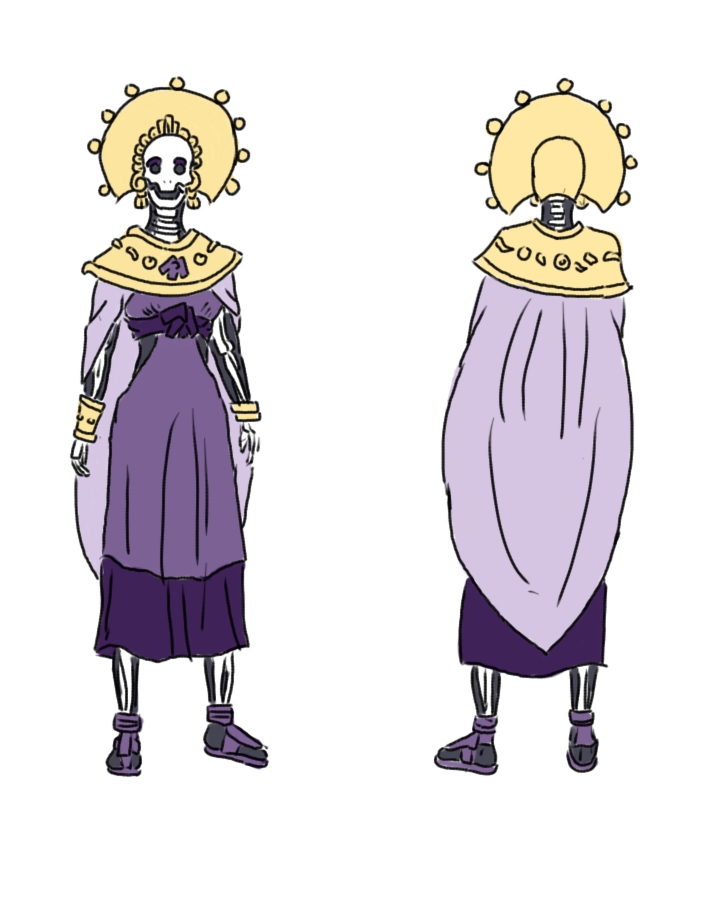
\includegraphics[height=0.3 \textheight]{Imagenes/reina_Mictla}
					\caption{Concepto de diseño de Mictecacihuatl.}
					\label{fig:MictecacihuatlDiseno}
	\end{figure}
\subsection{Concepto:}
\begin{itemize}
	\item \textbf{Historia antes del juego:}
	Nacida como la contraparte femenina de  Mictlantechtli, Mictecacíhuatl comprendio desde el inicio de su existencia cual era su rol como Diosa. Considerándose a sí misma como una reina que debía gobernar.  Mictecacíhuatl ejerce su gobierno sobre el Mictlán al tener la ultima palabra sobre los asuntos de mayor importancia, fungiendo como un puente que comunica el noveno nivel del Mictlán con el resto de los niveles y con los trece cielos.
	\\
	\par
	En diferentes ocasiones Mictecacíhuatl ha conspirado contra su esposo, llegando a enfrentarse a él para mantener el orden en el Mictlán; sus enfrentamientos siempre han surgido por la falta de liderazgo objetivo por parte de Mictlantechtli, ya que mientras  Mictlantechtli tiende a llevarse más por su orgullo y su temperamento a la hora de tomar decisiones, Mictecacíhuatl se guia más por un análisis de la situación.
	\item \textbf{Historia durante el juego:}
	Mictecacíhuatl ve con curiosidad el ataque de Xólotl, siendo la primera en darse cuenta que el ataque al Mictlán tenía connotaciones más fuertes de lo que parecían a primera instancia. A pesar de contar con todos los recursos para frenar a Xólotl, Mictecacíhuatl decide dejarlo avanzar, limitandose a cumplir con las ordenes de Mictlantechtli aun sabiendo que la estrategia de éste no era la más acertada. Ella deja que el Mictlán caiga pues confiaba plenamente en que en los trece cielos seran capaces de frenar a Xólotl, por lo que una vez vencido Xólotl y sin  Mictlantechtli, ella podría gobernar el Mictlán.
	item \textbf{Relaciones:}
	\begin{itemize}
		\item \textbf{Mictlantechtli:} Esposo de Mictecacíhuatl. Diversas malas decisiones que  Mictlantechtli ha tomado a lo largo de su gobierno en el Mictlán han llevado a Mictecacíhuatl a dejar de verlo como un líder (ver aparatado \ref{per:mictlantechtli}).  
		\item \textbf{Xólotl:} Persivido como un traidor,la presencia de Xólotl le permitirá a Mictecacíhuatl iniciar su propia misión para hacerse del control del Mictlán (ver aparatado \ref{per:xolotl}). 
	\end{itemize}                     
\end{itemize}

\subsection{Encuentro:}
\begin{itemize}
	\item Su primera aparición es en la cinemática 9 (ver aparatado \ref{Cin:Cinematica09}).
\end{itemize} 

\subsection{Habilidades:}
\begin{itemize}
	\item Mictecacíhuatl no es un jefe o enemigo a enfrentar por lo que no tiene una lista de habilidades a programar.
\end{itemize}  
\subsection{Armas:}
Sin armas.
\subsection{Ítems:}
Sin ítems
\subsection{Bloques de animación}
\begin{itemize}
	\item Animación normal.
	\item Animación caminar.
\end{itemize}